\section{Resistorn}
\textbf{HAREC a.\ref{HAREC.a.2.1}\label{myHAREC.a.2.1}}

\subsection{Allmänt}

Strömkretsar består av komponenter med olika egenskaper.
Den vanligaste egenskapen, åtminstone i likströmskretsar, är resistansen.
För att få avsedd funktion, så anpassar man resistansen i komponenterna.

\emph{Exempel}
En krets med strömkälla, lampa, kopplingsledningar och smältsäkring.
Kopplingsledningarna mellan komponenterna bör ha låg resistans och därför lågt
spänningsfall (små förluster). Lampan skall däremot ha hög resistans och därmed
höga förluster för att kunna bli het och lysa. Smältsäkringen skall skydda
ledningarna från för hög ström. Säkringen ges därför en resistans, som gör
att den smälter när strömmen överstiger ett tillåtet värde.
Som hjälpmedel för att fördela spänningar och strömmar i en krets, så används
en komponenttyp kallad \emph{resistor}. Dess utmärkande egenskap är
\emph{resistans} - även kallad ohmskt motstånd.

\subsection{Enheten Ohm}
\textbf{HAREC a.\ref{HAREC.a.2.1.1}\label{myHAREC.a.2.1.1}}

(Se även kapitel 1)

Resistansen mellan två punkter i en strömkrets är \(1 \Omega\) (uttalas
"en åm"), när spänningen mellan punkterna gör att en ström av 1 A (en ampere)
flyter i kretsen.

Inom elektroniken används höga resistansvärden och därför även följande
multipler av enheten
\begin{tabular}{lll}
  1 kiloohm & (\(1\ k\Omega\)) & = \(10^3\) Ohm \\
  1 megaohm & (\(1\ M\Omega\)) & = \(10^6\) Ohm \\
\end{tabular}

\subsection{Resistans i strömledare}
\textbf{HAREC a.\ref{HAREC.a.2.1.2}\label{myHAREC.a.2.1.2}}

För att bestämma resistansen, t. ex. i en tråd,
behöver man veta dess resistivitet, tvärsnittsyta, längd och temperatur.

\emph{Resistivitet}

Resistivitet är ett materials strömledningsegenskaper. Ett annat namn för
resistivitet är specifik resistans. Symbolen för resistivitet är \(\rho\)
(uttalas rå).

Formeln for resistivitet är \(\rho = \frac{ohm \cdot mm^2}{m}\)

Följande formel gäller för beräkning av resistansen i en strömledare med
linjär ström/spänningskaraktär.

\(R = \rho \frac{I}{A} \)

\(l\ [meter]\) \(A\ [mm^2]\) \(\left[\rho = \frac{\Omega \cdot A}{m} \right]\)

Exempel

\(l = 4\ m\) koppartråd

\(A = 2\ mm^2\)

\(\rho \text{ (koppar)} = 0.017\)

\(R = \rho \frac{I}{A}\) \(R = 0.017 \frac{4}{2} = 0.034\ \Omega\)

Not. Förväxla inte A [tvärsnittsytan] i denna formel med beteckningen A t. ex.
i Ohms lag då A betecknar strömstyrkan.

\subsection{Resistiva material}

Resistorer kan utföras med olika typer av resistiva material, vilket bestämmer
användningsområdet. En resistor, vars resistans är oberoende av ström, spänning
och annan yttre påverkan t.ex. temperatur och ljus, sägs ha linjär karaktär.
Om resistansen däremot beror av yttre påverkan, så sägs resistorn ha olinjär
karaktär. Man skiljer mellan tre huvudgrupper av resistiva material. Det kan
vara en kropp av pressat kol eller ett ledande ytskikt på ett isolerande
underlag eller metalltråd på en isolerande stomme. På senare tid har tillkommit
integrerade resistorer, d.v.s. flera resistorer av resistiva skikt på ett
gemensamt isolerande underlag. Här beskrivs i korthet resistortyper.
Se f.ö. leverantörskataloger.

\subsection{Utförandeformer}

Resistorer kan utföras med fast eller ställbart resistansvärde. Här följer
först en översikt över resistorer med olika resistiva material och fast
resistansvärde.

\subsection{Fasta resistorer med linjär karaktär}

\emph{Massaresistar}

Det resistiva materialet består av kolmassa med bindemedel (kolkomposit).
Massan är bakad till en stav eller ett rör. Anslutningsledningarna är inbakade
i materialet. Massaresistorer är lämpliga för lik- och växelströmskretsar med
låga krav på temperaturberoende och egenbrus. Den homogena kroppen gör att
egeninduktansen är låg. Å andra sidan uppstår vid höga frekvenser en
skineffekt, d.v.s. strömkoncentration vid ytan, som medför viss resistansökning.

\emph{Kolfilmsresistor}

Det resistiva materialet består av ett kolskikt, som genom förångning överförts
till ett keramiskt rör. Resistansen bestäms av tjockleken på skiktet samt av
spiralformade spår i detta. Genom spiraliseringen tillförs en induktans, men
som i någon mån uppvägs av egenkapacitansen.

\emph{Metallfilmresistor}

I denna typ är kolfilmen ersatt av ett metallskikt. Eftersom egenkapacitansen
är liten, så är typen lämpad för höga frekvenser.

\emph{Tjockfilmsresistor}

Det resistiva materialet består en film av bl. a. metalloxid, som screentrycks
på ett keramiskt underlag. Typen har god tålighet mot pulser och höga
temperaturer, men har relativt högt egenbrus. Ytmonterade resistorer är oftast
tillverkade av tjockfilm.

\emph{Tunnfilmsresistor}

Det resistiva materialet består av en tunn metallfilm, som genom förångning
överförts till ett underlag av glas eller keramik. Denna resistertyp har över
lag god stabilitet och används ofta i apparater med hög precision. Egenskaperna
vid höga frekvenser är dock inte så bra.

\emph{Metalloxidresistor}

Denna resistertyp har ett spiralformat skikt av metalloxid. Temperatur- och
spänningsberoendet är måttligt. Tåligheten mot pulser och höga temperaturer är
stor. Typen kan i någon mån ersätta trådlindade resistorer.

\emph{Resistornät}

Resistornät (integrerade resistorer) består av flera resistiva skikt på ett
gemensamt isolerande underlag, d.v.s. liknande teknik som för tjock- och
tunnfilmsresistorer.

\emph{Trådlindad resistor}

Det resistiva materialet är en metalltråd, som är lindad på en stomme som tål
hög temperatur; det kan var keramik, glas etc.
Tåligheten mot pulser och höga temperaturer är stor.

\subsection{Fasta resistorer med olinjär karaktär}
\textbf{HAREC a.\ref{HAREC.a.2.1.3}\label{myHAREC.a.2.1.3}}

Vanligast är att materialet i resistorer har linjär ström-/spänningskaraktär,
men det finns även sådana med olinjär karaktär. I resistorer med olinjär
karaktär är det ingående materialet av halvledartyp.

\emph{Spänningsberoende resistor - Voltage Dependent Resistar (VOR)}

Linjära resistorer påverkas knappast av den pålagda spänningen. Resistorer av
kiselkarbid har däremot en hög resistans vid låg spänning och omvänt en låg
resistans vid hög spänning. VOR används t.ex. för begränsning av
spänningstoppar.

\emph{Ljusberoende resistor, fotoresistor - Light Dependent Resistar (LDR)}

Ledningsförmågan i halvledare påverkas inte bara av värme utan även av ljus.
Halvledare av germanium och särskilt sammansatta halvledare av kadmiumoxid,
blysulfid och indiumantimonid har särskilt stor ljuskänslighet. Kadmiumsulfid
är känsligast för synligt ljus medan andra material är känsligast i det
infraröda området.

\emph{Magnetfältberoende resistor (fältplatta)}

Resistansen ökar med längden på strömledaren. Denna egenskap används i
magnetfältberoende fältplattor. En sådan består av en keramisk bärarplatta med
en yta av indiumantimon id. I ytan är ytterst smala parallella metallbanor
inlagda på ett avstånd av någon \(\mu m\). Normalt går strömmen kortaste vägen
tvärs över banorna, men när ett magnetfält träffar vinkelrätt mot plattans yta,
så avlänkas elektronerna. De får då längre väg över till nästa metallbana och
den totala resistansen ökar.

\emph{Temperaturberoende resistor}

Se nedan om NTC och PTC i resistorer.

\subsection{Temperaturkoefficienten för resistorer}

Resistansen i ingående material påverkas av temperaturen, varvid det skiljer
mellan materialen.

Amorft kol och de flesta halvledande materialleder bättre när de är varma- de
har en negativ temperaturkoefficient (NTC). Sådana material finns t. ex. i
dioder och transistorer.

Däremot leder metaller och speciella halvledarmaterial bättre när de är kalla -
de har en positiv temperaturkoefficient (PTC). Glödtråden i glödlampor och
elektronrör är resistorer med positiv temperaturkoefficient (PTC). I vissa
metallegeringar, som t.ex. i konstantan, kan resistansen till och med vara
nästan konstant vid varierande temperatur.

Alla material har en temperaturkoefficient, som anger hur mycket resistansen
ändras per grad. Resistansen vid någon annan temperatur kan därför beräknas med
följande formel, där man sätter in begynnelsetemperaturen [ \(\vartheta\) ]
(°C), temperaturändringen [ \(\Delta \vartheta\) ] och
temperaturkoefficienten [ \(\alpha\) ].

\(R_{varm} = R_{kall} \pm \alpha \cdot \Delta \vartheta \cdot R_{kall}\)

Resistansändringen är ledet

\( \Delta R = \pm \alpha \cdot \Delta \vartheta \cdot R_{kall}\)

Temperaturkoefficienten kan vara positiv (NTC) eller negativ (NTC).
I principscheman har PTC- respektive NTC-resistorer symboler som på bilden.

\begin{figure*}
\begin{center}
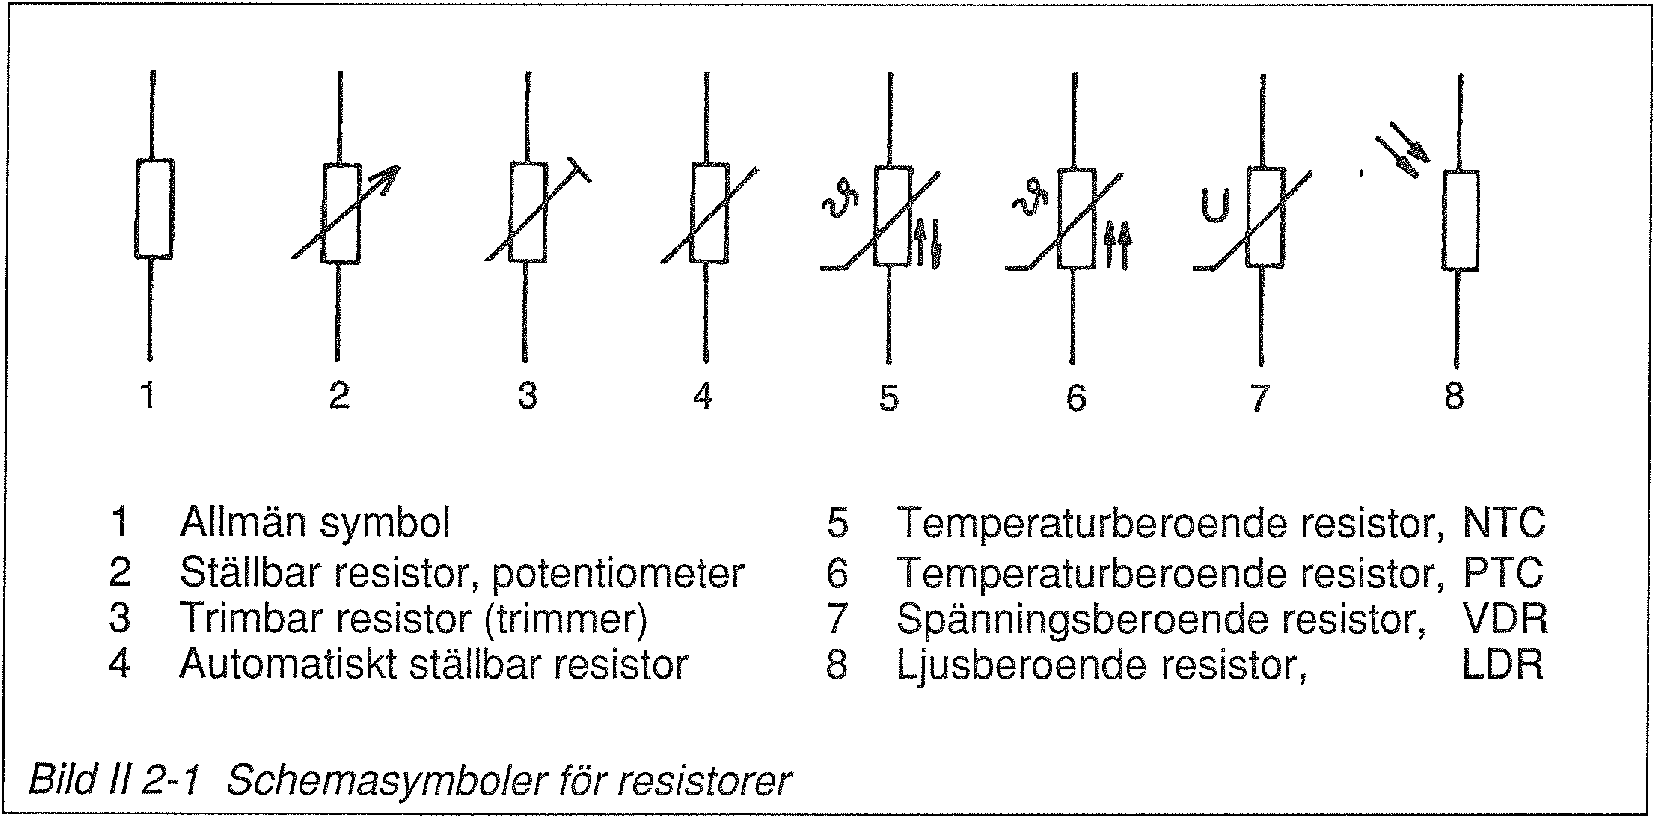
\includegraphics[width=14cm]{images/bild_2_2-01}
\caption{Schemasymboler för resistorer}
\label{fig:BildII2-1}
\end{center}
\end{figure*}

Bild \ref{fig:BildII2-1}

\subsection{Variabla resistorer}
En resister kan även utföras med variabelt resistansvärde. Då används endast
den andel av det resistiva materialet, som finns mellan en resistors ena ände
och ett uttag någonstans mellan ändarna. En sådan anordning kallas för reostat.
Om en variabel resistor används som spänningsdelare, så kallas den för
potentiometer.

I en potentiometer används dels hela resistansen mellan ändpunkterna och dels
andelen mellan uttaget och någon av ändpunkterna. Uttagets mekaniska utförande
beror oftast av hur bekvämt inställningen skall kunna ske. En potentiometer,
där det resistiva materialet är lagt på en cirkulär bana och uttaget är fäst
vid en axel i banans centrum, medger enkel inställning med mejsel, ratt etc.
Ett enklare slags uttag är en släpkontakt eller ett spännband som kan flyttas
utmed en stavformad resistor.

\subsection{Resistiva material i variabla resistorer}

Banan i en variabel resister består i princip av liknande resistiva material
som i en fast resistor. Billigast och enklast är en bana av kol, som är tryck
på ett enkelt underlag. Nackdelar är låg efekttålighet, dålig upplösning och
linjäritet, högt brus och kort livslängd. Fördelen är lågt pris.
Bättre än en kolbana är en bana av kolkomposit, d.v.s. kolpulver med bindemedel,
som är tryckt på ett underlag. Nackdel är högre pris och låg effekttålighet,
medan fördelarna är god upplösning, lågt brus och lång livslängd.
Vill man ha god effekttålighet och temperaturstabilitet, utöver kolkompositens
egenskaper, så erbjuder en bana av cermetsådana fördelar. En cermetbana består
av en blandning av metaller och keramik, som trycks på ett underlag.
Trådlindad bana har främst god tålighet mot hög effekt. Tålighet vid hög ström
genom uttaget är en nannan fördel.

\subsection{Linjära och olinjära patentiometrar}

En potentiometer har en kurvform, varvid avses resistansändringen som funktion
av uttagets rörelseväg utmed resistansbanan. Kurvformen kan utföras linjär,
logaritmisk etc. Olinjära kurvor består då oftast av en följd av linjära
segment, som tillsammans någorlunda motsvarar den önskade olinjära formen. Ett
exempel på det är när en kurvform anges som linjär/logaritmisk.

\subsection{Effektutveckling i resistorer}
\textbf{HAREC a.\ref{HAREC.a.2.1.4}\label{myHAREC.a.2.1.4}}

I resistorer utvecklas värme av den ström som flyter igenom. Värmeutvecklingen
sker enligt Joule's lag, som återges i kapitel 1. Hur mycket effekt i form av
värme som strålas ut från resistorn beror på storleken på dess yta och
egentemperatur samt på omgivningens temperatur. Det finns en övre gräns för hur
stor värme det ingående materialet tål innan det förstörs och eventuellt fattar
eld. En resistors effekttålighet framgår i vissa fall av påstämplade värden.
I övriga fall är man hänvisad till kataloguppgifter eller en bedömning, som ev.
kan grundas på höljets utseende och dimensioner.

\subsection{Standardiserade komponentvärden}

Resistorer tillverkas vanligen med standardiserade värden ur någon talserie.
Märkning av resistorer Resistorer märkas med huvuddata enligt något system av
siffror och bokstäver eller med en färgkod. Flera olika system tillämpas.
(Se f.ö. leverantörskataloger för information om komponentdata, märkning o.s.v.)
